\section{Design}
\label{sec:design}

\subsection{Overview}
\label{sec:design:overview}

The architecture of TrustFA is in Figure \ref{fig:arch}. We assume the
smartphone is running Android OS as the legacy OS. Besides the legacy OS in
TrustZone normal world, a secure kernel is placed in secure world. The secure
kernel can be either a customized Linux kernel or a new tiny kernel developed
from scratch (e.g., xv6 \cite{xv6}).  The device first boots into the secure
kernel in secure world which then boots the legacy OS in normal world. Touch
screen driver, display driver, crypto library and computer vision library (e.g.,
OpenCV) are ported to secure world kernel. A kernel module (tz.ko) is loaded in
normal world for the communication between two worlds.

\begin{figure}[htb]
	\centering
	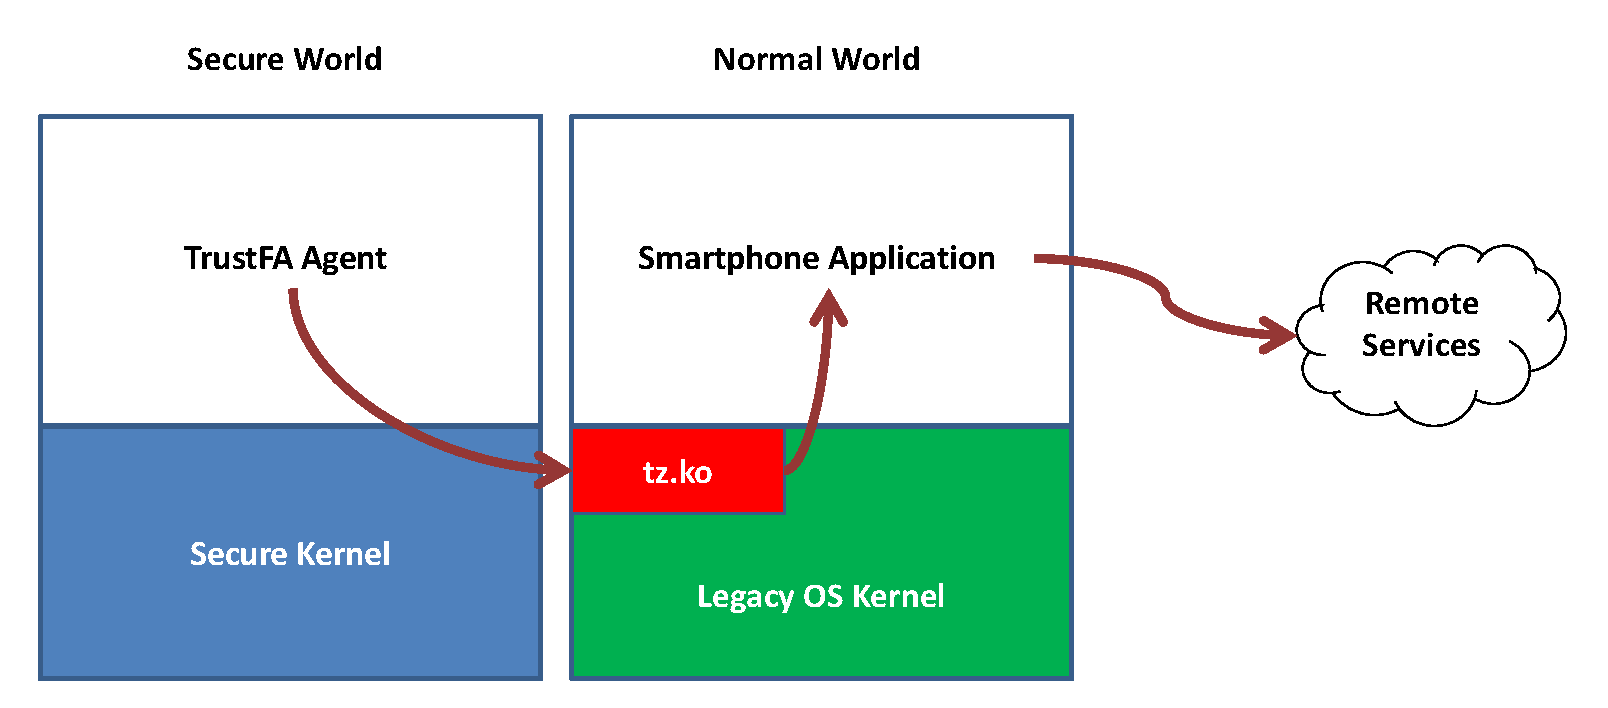
\includegraphics[width=1.0\columnwidth]{figures/arch.eps}
	\caption{TrustFA Architecture}
	\label{fig:arch}
\end{figure}

\begin{figure*}[htb]
	\centering
	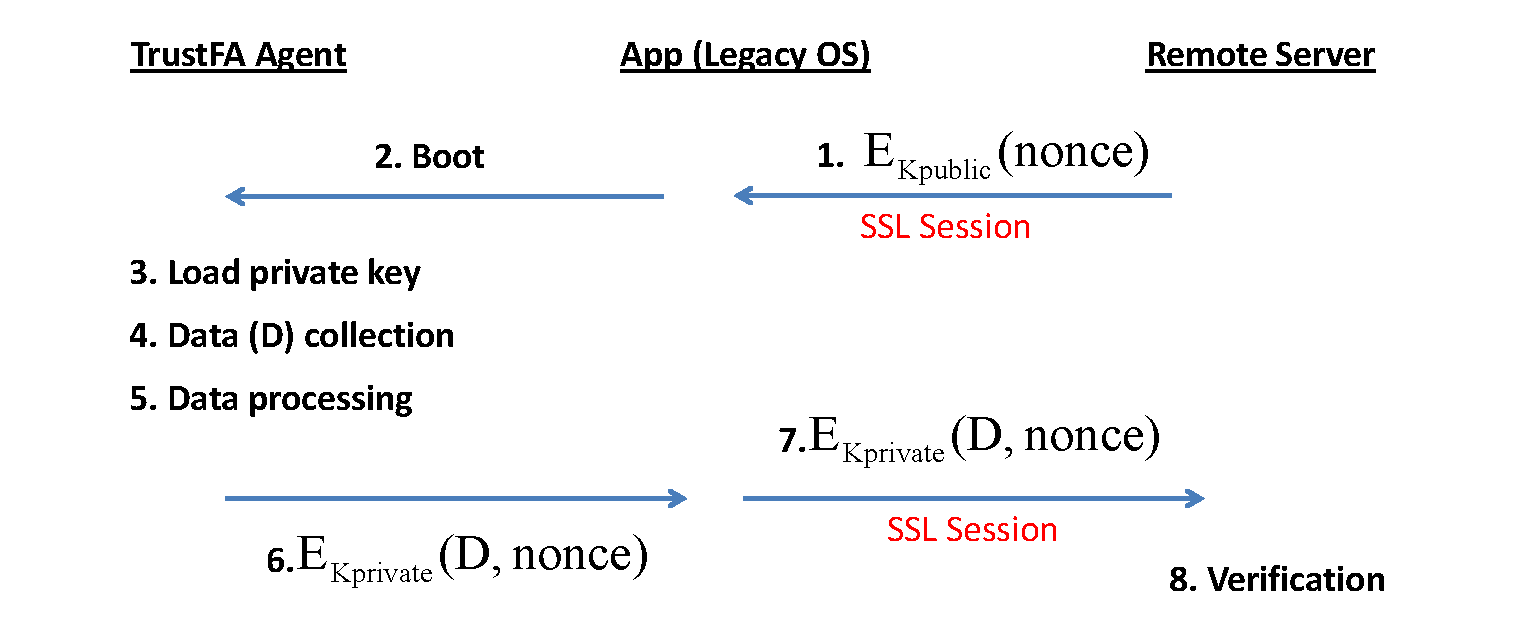
\includegraphics[width=2.0\columnwidth]{figures/authentication.eps}
	\caption{TrustFA Facial Authentication Workflow}
	\label{fig:authentication}
\end{figure*}

\noindent
{\bf Trust Model~}
Our trust model is rooted in the hardware isolation provided by the ARM
TrustZone. The TCB includes secure kernel and TrustFA Agent in secure world. We
assume the legacy OS is untrusted and can be potentially malicious. If the
legacy OS becomes compromised, the TrustZone ensures the integrity and
confidentiality of code and data residing in the secure world. Besides, we
assume the attacker is able to obtain the flat photo and video of user from social
networks to mount the 2D media attack..

Secure boot ensures that only the untampered image can pass the integrity check
of the chip and boot on the device (Section \ref{sec:implementation}).  The
device owns a device key $K_{DEV}$ which is flashed permanently on the one-time
programmable (OTP) fuses. Only secure world has access to fuses to retrieve
$K_{DEV}$. Besides, a key pair ($K_{public}$ and $K_{private}$) is generated.  $K_{public}$ is placed on the remote server provisioning the
service. $K_{private}$ is encrypted with $K_{DEV}$ (as
$E_{K_{DEV}}{(K_{private})}$) and stored on the persistent storage. The secure
kernel retrieves the encrypted $K_{private}$ (as $E_{K_{DEV}}{(K_{private})}$) via
the normal world legacy OS storage driver and decrypt it with $K_{DEV}$ in
secure world. As $K_{DEV}$ is only accessible in secure world, the legacy OS is
not able to obtain $K_{private}$ in normal world. 

\subsection{2D Media Attack}
\label{sec:design:phase1}

To differentiate the 3D face from 2D counterfeits, we leverage the solution in
\cite{Chen-Sensor} to correlate the camera with the accelerometer. As soon as
the authentication starts, the user moves the smartphone horizontally for a
short distance in front of the face from left to right. Once the face area is
greater or equal to 40\% area of the video frame, the smartphone starts sampling
video (from camera) and accelerations (from accelerometer). Once the face area
is smaller than 30\%, the sampling stops.

TrustFA Agent analyzes the sampled accelerations to calculate the time $t_l$ and
$t_r$ when the smartphone is on the left and right of the face respectively. The
video frames at $t_l$ (as $P(t_l)$), $t_r$ (as $P(t_r)$) and $t_m=(t_l+t_r)/2$
(as $P(t_m)$) are selected and processed. $P(t_l)$ and $P(t_r)$ are used as
input for Nose Angle Detection algorithm. The algorithm processes the two frames
and identify the nose's angle. The orientation of the angle is reversed when the
camera is moved horizontally in front of the face. If the input of camera is a
planar photo, the orientation change of nose angle will not happen. More details
of the algorithm are in \cite{Chen-Sensor}. If the input is not a 2D
counterfeit, TrustFA Agent will send $P(t_m)$ (or features extracted from $P(t_m)$) to the
remote server for authentication.

\subsection{Untrusted OS}
\label{sec:design:phase2}

When the legacy OS in normal world is compromised, the attacker is able to
tamper the camera/accelerometer data or provide a pre-recorded set of video/accelerations 
for authentication.  For the purpose of preventing this
attack, we leverage TrustZone to configure the camera and accelerometer as secure.
To reduce the code size of secure kernel, we will not implement the file system
and networking driver for it. 

To send data to the remote server over internet for
authentication, the secure kernel first encrypts the data with $K_{private}$ and
transfer the ciphertext to the normal world buffer. The normal world buffer is
allocated by the TrustZone driver (tz.ko) in normal world. The buffer can be
accessed by both secure world and normal world. Finally, the normal world legacy
OS will send the ciphertext to the remote server using its networking driver.

\subsection{TrustFA Authentication Workflow}

Figure \ref{fig:authentication} shows the workflow of TrustFA. We assume a
Android application wants to authenticate the user with TrustFA. To secure Phase
3, we assume an SSL session is established between the application and remote
server to transmit the data securely over internet.

The application first retrieves a nonce from server and boots TrustFA Agent with
the nonce in secure world. If $K_{private}$ is not in secure world, TrustFA
Agent obtains it via the legacy OS. In step 4, the user moves the smartphone in
front of the user's face to take video and accelerations as in section
\ref{sec:design:phase1}. In step 5, TrustFA Agent processes the accelerations
and extracts three photos $P(t_l)$, $P(t_r)$ and $P(t_m)$. If the input is not a
3D counterfeit, TrustFA will encrypt $P(t_m)$ (or its features) and the nonce
together as
$E_{K_{private}}(D, nonce)$. The ciphertext is then copied to the buffer in
normal world and forwarded to the remote server via SSL session in step 6 \& 7.
Finally, the server decrypts the ciphertext with $K_{public}$, check the nonce, and
authenticate the user. Once the user is authenticated, the server will send an
OAuth token to the application.
